% vim: spell spelllang=en:
%! TEX root = **/00-main.tex

\section{Profiling of clusters}%
\label{sec:profiling_of_clusters}

\newcommand{\profiling}[3]{
\begin{figure}[H]
    \centering
    \includegraphics[width=0.7\textwidth]{prof-c3-#1-#2}
    \caption{#3}%
    \label{fig:prof-#1-#2}
\end{figure}
}

\begin{figure}[H]
    \centering
    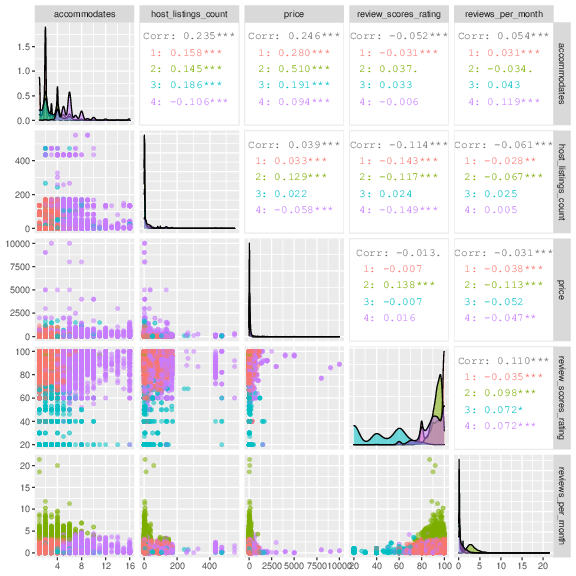
\includegraphics[width=0.9\textwidth]{pairs.png}
    \caption{Pair plot of some numerical variables}%
    \label{fig:pair}
\end{figure}

\Cref{fig:pair} shows a pair plot of the some numerical variables colored by clusters. We
can appreciate how the clusters
obtained relate to the numerical variables. In the following sections we discuss
these variables and some others in more extent.

% --- cat

\pagebreak

\profiling{host_is_superhost}{side}{Superhost distribution}
\profiling{host_since_year}{percent}{Host since year distribution}
In \cref{fig:prof-host_is_superhost-side} we can see how cluster 2 has a significantly higher proportional amount of superhosts when comparing to the rest of cluster, while cluster 3 has very few of them. This could indicate that hosts in cluster 2 are better hosts, with more experience and a pretty good record of dealing with clients. The hypothesis is confirmed by \Cref{fig:prof-host_since_year-percent}, where, comparing the same two clusters we see a tendency: cluster 2 is composed mostly of veteran hosts whereas cluster 3 is made up of more novice ones.
%\profiling{host_is_superhost}{stack}{}


%\profiling{host_response_time}{}{} %?


\clearpage
\subsection{Room Types \& Accommdates}%

%profiling{room_type}{percent}{room type bar}
%\profiling{room_type}{stack}{room type bar}


% --- num

%\clearpage
%\subsection{Accommodates}%

%\profiling{accommodates}{vi}{Accommodates}
%\profiling{accommodates}{bp}{Accommodates}
\profiling{accommodates}{meanp}{Accommodates}
\profiling{room_type}{side}{room type bar}
In \cref{fig:prof-accommodates-meanp} we can see that listings on cluster 4 accommodate
much more people than the ones in other clusters. By looking at \cref{fig:prof-room_type-side}, we can correlate this with the fact that most of the listings on cluster 4 are entire houses or apartments, that usually accommodate more people than hotel rooms, private rooms or shared rooms.

\clearpage
\subsection{Host listings count}%

\profiling{host_listings_count}{meanp}{Host listings count}
\profiling{host_listings_count}{bp}{Host listings count}
In \cref{fig:prof-host_listings_count-meanp,fig:prof-host_listings_count-bp} we can differences in the clusters.
Cluster 4 has the highest mean, followed by cluster 3. The other two seem to be quite
similar. It might indicate that the hosts of the listings in cluster number 4 are actually businesses.

\profiling{price}{meanp-tallat200}{Price}
\profiling{price}{vi-tallat200}{Price}
When looking at \cref{fig:prof-price-meanp-tallat200,fig:prof-price-vi-tallat200} we can clearly see that the listings in cluster 4 have an average price way higher that the other ones. As we already found out that cluster 4 contains the listings that accommodate more guests as well. This makes sense because a house that can accommodate more guests is expected to be more expensive.


\subsection{Review scores rating}%
\label{sub:prof-review_scores_rating}

\profiling{review_scores_rating}{meanp}{Review scores rating}
%\profiling{review_scores_rating}{vi}{Review scores rating}
\profiling{review_scores_rating}{bp}{Review scores rating}

Looking at \cref{fig:prof-review_scores_rating-meanp,fig:prof-review_scores_rating-bp} we can see that listings on cluster 3 have, on average, much lower review score rantings. The rest seem to have a really similar mean and variance. We can conclude that cluster 3 contains the bad reviews while high reviews seem to distribute between the others.

\clearpage
\subsection{Reviews per month}%

\profiling{reviews_per_month}{meanp}{Reviews per month}
%\profiling{reviews_per_month}{vi}{Reviews per month}
\profiling{reviews_per_month}{bp}{Reviews per month}

\Cref{fig:prof-reviews_per_month-bp,fig:prof-reviews_per_month-meanp} show that listings in cluster 2 average a lot more reviews per month and that listings in
cluster 3 have the least amount. This makes sense because, as we have already seen, the reviews' score is directly correlated of the number of reviews, and given that the listings on cluster 3 have a pretty bad review score, they had to have a small amount of reviews.



% Profiling of clusters: Use class variable as a response variable to analyze
% conditional distributions of variables to clusters and eventual statistical
% tests to assess which variables are significant in each cluster. Detect
% commonalities of each cluster and differences between clusters. What is
% intrinsic of each cluster? What distinguishes clusters among them?

% Profiling graphs, CPGs, multiple boxplots, bivariate barplots, descriptive by
% groups, etc...

% For selected relevant variables, you can also add specific profiling tests to
% complete clusters interpretation

% Synthesize the result of the classes’ interpretation process into a set of
% templates characterizing the clusters, one template per cluster
